\documentclass{article}
\usepackage[T1]{fontenc}
\usepackage{lmodern}
\usepackage{graphicx}
\usepackage{amsmath,amssymb}
\usepackage[a4paper,margin=2cm]{geometry}
\usepackage[absolute,overlay]{textpos}
\setlength{\TPHorizModule}{1mm}
\setlength{\TPVertModule}{1mm}
\usepackage[indonesian]{babel}
\usepackage{hyperref}
\setlength{\emergencystretch}{2em}
% unit: Halaman 105

\begin{document}

% === Halaman 105 (llm) ===

\vspace{243.54mm}

Demo Hill Cipher online: https://www.dcode.fr/hill-cipher

% deskripsi: Screenshot antarmuka situs dCode untuk alat Hill Cipher, menunjukkan input ciphertext, matriks kunci 2x2, opsi alfabet, dan area hasil enkripsi/dekripsi.
% bbox normalisasi: [0.6700, 0.1400, 0.9400, 0.9600]
\begin{textblock*}{56.70mm}(140.70mm,41.58mm)
\noindent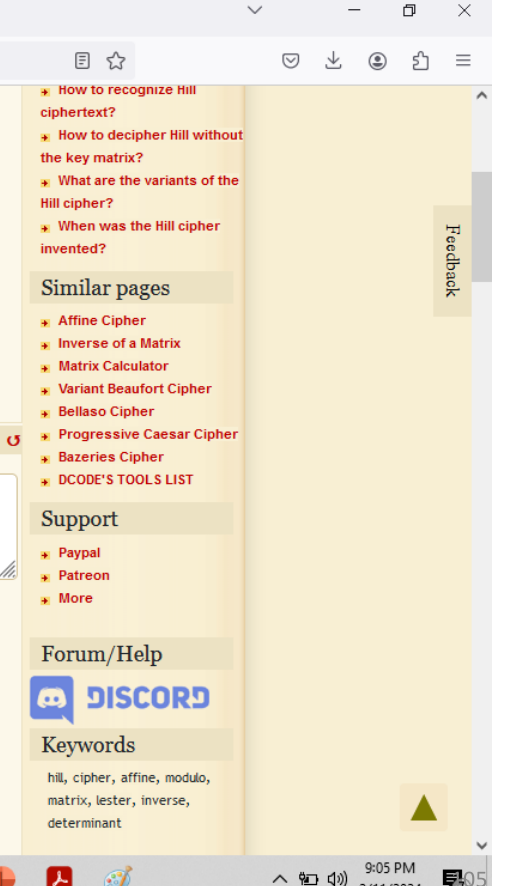
\includegraphics[width=56.70mm,height=243.54mm]{../../images/llm/page_105_img_01.png}%
\end{textblock*}

\end{document}
